% Options for packages loaded elsewhere
\PassOptionsToPackage{unicode}{hyperref}
\PassOptionsToPackage{hyphens}{url}
%
\documentclass[
  12pt,
]{article}
\usepackage{lmodern}
\usepackage{amsmath}
\usepackage{ifxetex,ifluatex}
\ifnum 0\ifxetex 1\fi\ifluatex 1\fi=0 % if pdftex
  \usepackage[T1]{fontenc}
  \usepackage[utf8]{inputenc}
  \usepackage{textcomp} % provide euro and other symbols
  \usepackage{amssymb}
\else % if luatex or xetex
  \usepackage{unicode-math}
  \defaultfontfeatures{Scale=MatchLowercase}
  \defaultfontfeatures[\rmfamily]{Ligatures=TeX,Scale=1}
\fi
% Use upquote if available, for straight quotes in verbatim environments
\IfFileExists{upquote.sty}{\usepackage{upquote}}{}
\IfFileExists{microtype.sty}{% use microtype if available
  \usepackage[]{microtype}
  \UseMicrotypeSet[protrusion]{basicmath} % disable protrusion for tt fonts
}{}
\makeatletter
\@ifundefined{KOMAClassName}{% if non-KOMA class
  \IfFileExists{parskip.sty}{%
    \usepackage{parskip}
  }{% else
    \setlength{\parindent}{0pt}
    \setlength{\parskip}{6pt plus 2pt minus 1pt}}
}{% if KOMA class
  \KOMAoptions{parskip=half}}
\makeatother
\usepackage{xcolor}
\IfFileExists{xurl.sty}{\usepackage{xurl}}{} % add URL line breaks if available
\IfFileExists{bookmark.sty}{\usepackage{bookmark}}{\usepackage{hyperref}}
\hypersetup{
  pdftitle={Turnout and Amendment 4: Mobilizing Eligible Voters Close to Formerly Incarcerated Floridians},
  pdfauthor={Kevin Morris ,},
  hidelinks,
  pdfcreator={LaTeX via pandoc}}
\urlstyle{same} % disable monospaced font for URLs
\usepackage[margin=1in]{geometry}
\usepackage{longtable,booktabs}
\usepackage{calc} % for calculating minipage widths
% Correct order of tables after \paragraph or \subparagraph
\usepackage{etoolbox}
\makeatletter
\patchcmd\longtable{\par}{\if@noskipsec\mbox{}\fi\par}{}{}
\makeatother
% Allow footnotes in longtable head/foot
\IfFileExists{footnotehyper.sty}{\usepackage{footnotehyper}}{\usepackage{footnote}}
\makesavenoteenv{longtable}
\usepackage{graphicx}
\makeatletter
\def\maxwidth{\ifdim\Gin@nat@width>\linewidth\linewidth\else\Gin@nat@width\fi}
\def\maxheight{\ifdim\Gin@nat@height>\textheight\textheight\else\Gin@nat@height\fi}
\makeatother
% Scale images if necessary, so that they will not overflow the page
% margins by default, and it is still possible to overwrite the defaults
% using explicit options in \includegraphics[width, height, ...]{}
\setkeys{Gin}{width=\maxwidth,height=\maxheight,keepaspectratio}
% Set default figure placement to htbp
\makeatletter
\def\fps@figure{htbp}
\makeatother
\setlength{\emergencystretch}{3em} % prevent overfull lines
\providecommand{\tightlist}{%
  \setlength{\itemsep}{0pt}\setlength{\parskip}{0pt}}
\setcounter{secnumdepth}{5}
\usepackage{rotating}
\usepackage{setspace}
\usepackage{lineno}
\linenumbers
\usepackage{booktabs}
\usepackage{longtable}
\usepackage{array}
\usepackage{multirow}
\usepackage{wrapfig}
\usepackage{float}
\usepackage{colortbl}
\usepackage{pdflscape}
\usepackage{tabu}
\usepackage{threeparttable}
\usepackage{threeparttablex}
\usepackage[normalem]{ulem}
\usepackage{makecell}
\usepackage{xcolor}
\ifluatex
  \usepackage{selnolig}  % disable illegal ligatures
\fi
\newlength{\cslhangindent}
\setlength{\cslhangindent}{1.5em}
\newlength{\csllabelwidth}
\setlength{\csllabelwidth}{3em}
\newenvironment{CSLReferences}[2] % #1 hanging-ident, #2 entry spacing
 {% don't indent paragraphs
  \setlength{\parindent}{0pt}
  % turn on hanging indent if param 1 is 1
  \ifodd #1 \everypar{\setlength{\hangindent}{\cslhangindent}}\ignorespaces\fi
  % set entry spacing
  \ifnum #2 > 0
  \setlength{\parskip}{#2\baselineskip}
  \fi
 }%
 {}
\usepackage{calc}
\newcommand{\CSLBlock}[1]{#1\hfill\break}
\newcommand{\CSLLeftMargin}[1]{\parbox[t]{\csllabelwidth}{#1}}
\newcommand{\CSLRightInline}[1]{\parbox[t]{\linewidth - \csllabelwidth}{#1}\break}
\newcommand{\CSLIndent}[1]{\hspace{\cslhangindent}#1}

\title{Turnout and Amendment 4: Mobilizing Eligible Voters Close to Formerly Incarcerated Floridians\thanks{I am grateful to the editors and three anonymous reviewers for their helpful feedback and guidance. I would also like to thank Myrna Pérez, Patrick Berry, Peter Miller, Lia Merivaki, Lucia Trimbur, and participants at the 2021 Annual Meeting of the Southern Political Science Association for their comments and suggestions on this project. All errors are my responsibility.}}
\author{Kevin Morris\footnote{Researcher, Brennan Center for Justice at NYU School of Law, 120 Broadway Ste 1750, New York, NY 10271 (\href{mailto:kevin.morris@nyu.edu}{\nolinkurl{kevin.morris@nyu.edu}})} \textsuperscript{,}\footnote{PhD Student, Sociology Program, CUNY Graduate Center}}
\date{February 09, 2021}

\begin{document}
\maketitle
\begin{abstract}
Recent scholarship shows that eligible voters in neighborhoods home to many arrested and incarcerated individuals vote at lower rates than those in less-impacted neighborhoods. Little work, however, has interrogated how this turnout gap might be counteracted. This paper uses Amendment 4, a 2018 Florida ballot initiative that promised to re-enfranchise most individuals whose voting rights had been revoked due to a felony conviction, to investigate whether this turnout disparity can be narrowed by a ballot initiative of particular significance to communities most impacted by incarceration. Using prison release records, I identify the neighborhoods and households where formerly incarcerated individuals live and assess the voting history of their neighbors and housemates. I find no evidence that Amendment 4 increased these voters' turnout in 2018 relative to other voters. While ending felony disenfranchisement is necessary, closing the turnout gap resulting from histories of policing and incarceration will require greater investment and engagement.
\end{abstract}

\pagenumbering{gobble}
\pagebreak

\pagenumbering{arabic}
\doublespacing

\hypertarget{introduction}{%
\subsection*{Introduction}\label{introduction}}
\addcontentsline{toc}{subsection}{Introduction}

On November 6\textsuperscript{th}, 2018, Floridians voted to amend their state constitution to re-enfranchise individuals with felony convictions in their past (\protect\hyperlink{ref-Taylor2018}{Taylor 2018}). The move was hailed as transformative for Floridian --- and American --- democracy; \protect\hyperlink{ref-sentencing_2016}{Uggen, Larson, and Shannon} (\protect\hyperlink{ref-sentencing_2016}{2016}) had estimated a few years earlier that some 1.5 million Floridians were disenfranchised and had finished serving their sentences, making the amendment the largest expansion of the franchise in the United States since the Twenty-sixth Amendment lowered the voting age to 18. The amendment received broad support. Although it needed just 60 percent of the vote to pass, 64.5 percent of voters supported the ballot initiative. This support contrasts sharply with other statewide races: Ron DeSantis won the gubernatorial race with only 49.6 percent of the vote, while winning just 50.1 percent sent Rick Scott to the United States Senate.

Prior to 2018, Floridians convicted of felony offenses were permanently disenfranchised unless they applied for and received an individual pardon from the state's clemency board. This was characterized by a ``low success rate, cumbersome process, and lengthy amount of time'' (\protect\hyperlink{ref-Miller2012a}{B. L. Miller and Spillane 2012b, 432}) and was driven in part by gubernatorial discretion: although Charlie Crist restored voting rights to roughly 150 thousand individuals over a 4 year period, Rick Scott did so for fewer than 3 thousand people over 8 years (\protect\hyperlink{ref-Schlakman2018}{Schlakman 2018}). At the time Amendment 4 was passed, it was widely reported that the backlog of applications was nearly 10,000 and the wait stretched for as long as a decade (\protect\hyperlink{ref-Ramadan2018}{Ramadan, Stucka, and Washington 2018}). Over the years, Florida's procedure was subject to numerous lawsuits, and was ruled unconstitutional in early 2018 with Judge Mark Walker describing it as ``a gauntlet of constitutionally infirm hurdles.''\footnote{Hand et al.~v. Scott et al., 4:17cv128-MW/CAS (U.S. District Court for the Northern District of Florida 2018).} Amendment 4 promised to automatically restore voting rights once individuals had completed their sentence, though it did not apply to individuals convicted of murder or sexual offenses.

In recent years scholars have leveraged administrative records and sophisticated statistical techniques to study the actual political effects of felony disenfranchisement in the United States (e.g. \protect\hyperlink{ref-Meredith2014}{Meredith and Morse 2014}, \protect\hyperlink{ref-Meredith2015}{2015}; \protect\hyperlink{ref-Colgan2019}{Colgan 2019}; \protect\hyperlink{ref-Morris2021}{Morris 2021}). With the notable exception of \protect\hyperlink{ref-White2019a}{White} (\protect\hyperlink{ref-White2019a}{2019a}), however, the behavior of voters who live with individuals who have been convicted of felony offenses --- but have not themselves been convicted --- has gone unstudied. This article brings together these analytical approaches and an interdisciplinary body of literature to understand the political behavior of citizens whose family members have been incarcerated due to a felony conviction.

This study explores whether the opportunity to vote on Amendment 4 increased the (relative) participation among eligible voters who lived with or near individuals disenfranchised due to a period of felony incarceration. Americans' political knowledge is deeply shaped by the incarceration of a loved one (\protect\hyperlink{ref-Lee2014}{Lee, Porter, and Comfort 2014}), and exposure to the carceral state chills political involvement even among individuals who are not convicted. The criminal justice system can leave even would-be voters without a criminal record feeling as though political involvement is not for ``people like me,'' often despite having considerable political knowledge (\protect\hyperlink{ref-Lerman2014}{Lerman and Weaver 2014}). A growing body of quantitative research captures these ``spillover'' effects, demonstrating that neighborhoods with high levels of incarceration and disenfranchisement vote at markedly lower rates than other similar neighborhoods (e.g. \protect\hyperlink{ref-Burch2014}{Burch 2014}; \protect\hyperlink{ref-Morris2020}{Morris 2020}).

Amendment 4 in Florida offers a unique opportunity to investigate whether these chilling effects can be overcome by one ballot initiative. As I explain in the section that follows, Amendment 4 offered individuals living with or near formerly incarcerated individuals an opportunity to redefine their relationship with the government in positive ways. Although this made the ballot initiative perhaps particularly salient for these individuals, it took place against the backdrop of an entrenched carceral state that negatively structured many facets of their lives (see, for instance, \protect\hyperlink{ref-Travis2003}{Travis and Waul 2003}). Ultimately, I do not find evidence that Amendment 4 mobilized individuals living with or near formerly incarcerated Floridians in 2018 above-and-beyond turnout increases observed in other, similar voters.

\hypertarget{theory-and-literature}{%
\subsection*{Theory and Literature}\label{theory-and-literature}}
\addcontentsline{toc}{subsection}{Theory and Literature}

In recent years scholars have documented the effect of the American criminal legal system on the lives of those who come under its purview, even once they are no longer under formal supervision. The growth of the criminal legal system has resulted in what Monica Bell calls \emph{legal estrangement}, which reflects both \emph{legal cynicism} --- a cultural orientation that views the law and its enforcers as ``illegitimate, unresponsive, and ill equipped to ensure public safety'' (\protect\hyperlink{ref-Kirk2011a}{Kirk and Papachristos 2011, 1191}; see also \protect\hyperlink{ref-Sampson1998}{Sampson and Bartusch 1998}; \protect\hyperlink{ref-Kirk2011}{Kirk and Matsuda 2011}; \protect\hyperlink{ref-Morenoff2014}{Morenoff and Harding 2014}) --- and the objective structural conditions (such as policing practices and criminal law) that give rise to this orientation (\protect\hyperlink{ref-Bell2017}{Bell 2017, 2066} -- 2067). Legal estrangement has also been linked with ``institutional'' or ``system avoidance.'' Brayne (\protect\hyperlink{ref-Brayne2014}{2014, 385}), for instance, documents that ``individuals who have been stopped, arrested, convicted, or incarcerated are less likely to interact with institutions that keep formal records, such as hospitals, banks, employment, and schools.'' \protect\hyperlink{ref-Haskins2017}{Haskins and Jacobsen} (\protect\hyperlink{ref-Haskins2017}{2017}) finds that institutional avoidance explains formerly incarcerated men's reduced willingness to be involved with their children's schools, and \protect\hyperlink{ref-Remster2018}{Remster and Kramer} (\protect\hyperlink{ref-Remster2018}{2018}) shows that this avoidance explains the behavior of Black and non-Black individuals alike.

Institutional avoidance is especially clear when it comes to democratic participation, particularly in the voting booth. It is well established that a criminal conviction --- and, more specifically, a period of incarceration --- decreases turnout even when individuals are no longer legally disenfranchised (\protect\hyperlink{ref-Weaver2010}{Weaver and Lerman 2010}; \protect\hyperlink{ref-Burch2011}{Burch 2011}; \protect\hyperlink{ref-White2019}{White 2019b}; but see \protect\hyperlink{ref-Gerber2017}{Gerber et al. 2017}). The effect of disenfranchisement policy on the political behavior of individuals who experience the criminal justice system indirectly via the conviction of a family or community member, however, is somewhat mixed. Most research finds that turnout is measurably lower in states with stricter voter disenfranchisement policies or more disenfranchised citizens (e.g. \protect\hyperlink{ref-Bowers2009}{Bowers and Preuhs 2009}; \protect\hyperlink{ref-King2016}{King and Erickson 2016}), though \protect\hyperlink{ref-Miles2004}{Miles} (\protect\hyperlink{ref-Miles2004}{2004}) argues that these effects are small. The little research that has explored the spillover effects of disenfranchisement policy at the \emph{neighborhood} level has similarly found evidence that incarceration and disenfranchisement demobilizes eligible voters in impacted communities (\protect\hyperlink{ref-Burch2014}{Burch 2014}; \protect\hyperlink{ref-Morris2020}{Morris 2020}; but see \protect\hyperlink{ref-White2019a}{White 2019a}). Understanding whether Amendment 4 was likely to recoup the lost turnout of eligible voters who lived with or near the disenfranchised requires understanding \emph{how} their indirect exposure to the criminal justice system (or ``proximal contact'' (\protect\hyperlink{ref-Walker2014}{Walker 2014})) depressed turnout to begin with.

Work from Vesla Weaver and Amy Lerman (\protect\hyperlink{ref-Weaver2010}{2010}; \protect\hyperlink{ref-Lerman2014}{2014}) describes in great detail how legal estrangement ruptures individuals' willingness to engage in electoral politics. They argue that a felony conviction serves as ``a durable constraint and marker of their citizenship'' (\protect\hyperlink{ref-Lerman2014}{Lerman and Weaver 2014, 133}), and that custodial citizens --- individuals in communities with aggressive crime control who may or may not have a criminal history themselves --- ``become less likely to believe that they (and those like them) can change \emph{the system}, a reduction in external efficacy'' (\protect\hyperlink{ref-Lerman2014}{Lerman and Weaver 2014, 137}, emphasis in the original). Their work is replete with examples of individuals who know much about politics yet choose to ``stay below the radar'' because ``\,`they're {[}government officials{]} not interested in what I have to say'\,'' (\protect\hyperlink{ref-Lerman2014}{Lerman and Weaver 2014, 210}).

Importantly, these demobilizing consequences are not limited to those who are convicted; rather, ``the sense of alienation in a carceral regime emanates not only from what police might do to `you,' but from what they might do to your friends, your intimate partners, your parents, your children; to people of your race or social class; and to people who live in the neighborhood or the city where you live'' (\protect\hyperlink{ref-Bell2017}{Bell 2017, 2058}). Put differently, the legal system serves as a site of political socialization even for those who are not formally convicted of a crime (\protect\hyperlink{ref-Lee2014}{Lee, Porter, and Comfort 2014}; \protect\hyperlink{ref-Comfort2016}{Comfort 2016}; \protect\hyperlink{ref-Kirk2016}{Kirk 2016}). There is, however, some evidence that these chilling effects on political participation can be overcome. Recent work demonstrates that direct and indirect contact with the criminal justice system can be mobilizing when these experiences are linked with narratives of injustice (\protect\hyperlink{ref-Walker2017}{Walker and García-Castañon 2017}; \protect\hyperlink{ref-Walker2020}{Walker 2020}).

Of course, there is no bright line dividing individuals with \emph{indirect} exposure to the criminal justice system from individuals with their own, \emph{direct} exposure to the carceral state. The geographic concentration of policing and incarceration patterns (e.g. \protect\hyperlink{ref-Gelman2007}{Gelman, Fagan, and Kiss 2007}) mean that individuals in community with the formerly incarcerated --- that is, people living with or near formerly incarcerated residents --- might also have other, direct relationships with the criminal justice system. In 2017 there were 711,831 arrests in Florida but just 134,554 guilty felonious dispositions.\footnote{See \url{http://edr.state.fl.us/Content/resource-demand/criminal-justice/reports/criminal-justice/cj7.pdf}.} Although individuals who were arrested but not convicted of felonies were not legally disenfranchised, even low-level interactions can have a chilling effect on one's relationship with the government, a relationship Amendment 4 could have led them to reconsider.

Based on these literatures, I hypothesized that both the substance of the proposed constitutional amendment and the messaging used by the campaign supporting its passage would increase the relative turnout of individuals living with and near formerly incarcerated Floridians. Restoring voting rights to individuals who had been convicted of felony offenses would end the ``civil death'' of felony disenfranchisement (\protect\hyperlink{ref-Ewald2002}{Ewald 2002}; \protect\hyperlink{ref-Miller2012}{B. L. Miller and Spillane 2012a}), nullifying one of the durable badges identified by Lerman and Weaver. Amendment 4 offered those in community with the formerly incarcerated the chance to affirm that their family and community members deserved to have their voices heard in the democratic arena, a chance I anticipated would disproportionately spur them to participate.

Moreover, the public messaging employed by the Amendment 4 campaign was explicitly designed to change how voters understood the citizenship of disenfranchised individuals. The campaign cast the ballot initiative as an issue of fairness, criticizing Florida's existing disenfranchisement policy for creating two tiers of citizenship. The organization leading the campaign leveraged the notion that disenfranchised citizens deserved to be re-incorporated into the body politic in its very name --- ``Second Chances Florida.'' The framing was effective: the editorial boards of each of Florida's three biggest newspapers endorsed the amendment, all using language related to fairness and civic redemption. The Tampa Bay Times told readers they had a ``remarkable opportunity to remedy that unfairness'' (\protect\hyperlink{ref-tampabaytimes2018}{\emph{Tampa Bay Times} 2018}); the Sun Sentinel informed voters ``{[}t{]}here may never be an opportunity to do a better thing than to vote yes on this reform'' (\protect\hyperlink{ref-SunSentinelEditorial2018}{\emph{Sun Sentinel} 2018}); and the Orlando Sentinel said that Florida's then-policy ``denie{[}d{]} our fellow citizens a second chance. It denie{[}d{]} redemption'' (\protect\hyperlink{ref-ORLANDOSENTINEL2018}{\emph{Orlando Sentinel} 2018}). Insofar as the campaign was successful at helping these individuals understand the experiences of their formerly incarcerated family and community members in the context of a broader narrative of (racial) injustice, I expected this framing would mobilize them to vote at higher rates than other voters.

In addition to newspapers across the state, the campaign deployed ``volunteers from a broad coalition that included advocacy groups, Christian organizations, the League of Women Voters, criminal justice experts and, of course, those who had been convicted of felonies'' (\protect\hyperlink{ref-Robles2018}{Robles 2018}). Andrew Gillum, the Democratic gubernatorial candidate, also vocally supported the amendment, openly discussing his family's relationship with the criminal justice system and his own sibling's disenfranchisement (\protect\hyperlink{ref-Smith2018}{Smith 2018}). Voters were thus getting cues from all sorts of messengers that Amendment 4 deserved to be passed, and that individuals with convictions in their past should be allowed to vote. I expected that these cues, plus the descriptive representation (\protect\hyperlink{ref-Merolla2013}{Merolla, Sellers, and Fowler 2013}) promised by Gillum, would have proved especially mobilizing for the population in closest contact with disenfranchised Floridians.

At the same time, there was some reason to think the ballot initiative would not disproportionately increase turnout among voters in close contact with formerly incarcerated, disenfranchised individuals. Legal estrangement runs deep: the ``hidden curriculum'' of the criminal justice system (\protect\hyperlink{ref-Justice2014}{Justice and Meares 2014}; \protect\hyperlink{ref-Meares2017}{Meares 2017}) teaches individuals their place in this system over a very long period, through both incarceration and day-to-day interactions with government representatives such as the police. It is perhaps naive to expect that a single ballot initiative could overcome these negative forces.

Moreover, the individuals in these neighborhoods were perhaps less familiar with the content of Amendment 4 than others: \protect\hyperlink{ref-Bowler1994}{Bowler and Donovan} (\protect\hyperlink{ref-Bowler1994}{1994}), for instance, demonstrates that education and polarization are strong predictors of individuals' familiarity with ballot initiatives. \protect\hyperlink{ref-Shaker2012}{Shaker} (\protect\hyperlink{ref-Shaker2012}{2012}) also finds that higher-educated individuals are more knowledgeable about local politics. Given that formerly incarcerated individuals leave prison for neighborhoods with less access to higher education (see Table \ref{tab:demos} below), their neighbors and housemates may have been less aware of the amendment in the first place, in which case it obviously could not heighten motivation to cast a ballot.

\hypertarget{research-design-and-expectations}{%
\subsection*{Research Design and Expectations}\label{research-design-and-expectations}}
\addcontentsline{toc}{subsection}{Research Design and Expectations}

I begin by testing whether a neighborhood's formerly incarcerated population influenced its turnout in 2018. Because statewide felony probation records are not available, this analysis is based on only the subset of disenfranchised individuals who were imprisoned for a felony conviction. Neighborhoods that are home to formerly incarcerated individuals are identified by geocoding release records from the Florida Department of Corrections, and I offer two definitions of neighborhoods.

Neighborhoods are first defined as voting precincts. The Florida Division of Elections makes election results available at this level, which allows me to test turnout specifically on Amendment 4 and neighborhood-level support for the amendment. I can also assess how salient the amendment was for participants by estimating the share of voters who ``rolled off'' (or chose not to vote) for Amendment 4. Unfortunately, the use of precinct-level data leaves us with a major drawback: when doing analysis at this level, bias-free turnout denominators are hard to come by. Because the Census Bureau does not produce population estimates for individual voting precincts, turnout cannot be calculated by dividing the number of ballots cast by the eligible population (that is, citizens over the age of 17 without a felony conviction); rather, it must be constructed as a share of registered voters. If there is a relationship between the number of formerly incarcerated residents and the registration rate of a neighborhood, our estimates will be biased.

That could be the case in the study at hand. Some political organizers supporting Amendment 4 focused on canvassing neighborhoods with many formerly incarcerated individuals (\protect\hyperlink{ref-Speri2018}{Speri 2018}), potentially raising the registration rate in these areas. If relatively few of these newly-registered individuals voted, the net effect would be higher turnout among \emph{eligible residents} but lower turnout among \emph{registered voters}. For further discussion of how improper denominators can bias turnout estimates, see \protect\hyperlink{ref-Amos2017}{Amos, McDonald, and Watkins} (\protect\hyperlink{ref-Amos2017}{2017}) and \protect\hyperlink{ref-Amos2020}{Amos and McDonald} (\protect\hyperlink{ref-Amos2020}{2020}).

To address this potential problem, I also define neighborhoods as Census block groups. The Census Bureau makes estimates of the citizen voting-age population (a better denominator for turnout) available at this level. In this case, however, I must use a geocoded voter file to determine turnout. Because I aggregate the number of participants in a block group from individual-level data, I cannot determine whether an individual actually participated in the contest for Amendment 4 or they rolled off. Similarly, I am unable to interrogate the relationship between block group characteristics and support for Amendment 4. Although each definition of neighborhood presents some drawbacks, the two definitions together paint a full picture.

After examining whether the presence of formerly incarcerated residents was related with neighborhoods' voting behavior, I ask whether voters who lived with formerly incarcerated individuals turned out at higher rates in 2018. For this analysis, I use the release addresses of formerly incarcerated individuals (the most recent address available, according to the Department of Corrections) and voter file data to identify registered voters who lived with formerly incarcerated individuals. Voters are considered ``treated'' if they lived with a formerly incarcerated individual, and ``untreated'' otherwise. I then use a variety of individual- and neighborhood-level characteristics to match treated and untreated voters using what methodologists call a ``genetic'' process (\protect\hyperlink{ref-Sekhon2011}{Sekhon 2011}).

After matching these voters, I employ a difference-in-differences specification to determine whether treated voters participated at higher rates in the 2018 election. These analyses are run for all voters who lived with a formerly incarcerated individual, as well as only the subset of households whose members have not been to prison for many years. This final specification allows me to disentangle the depressive effect of indirect exposure to the criminal justice system from the mobilizing effect of Amendment 4 in 2018 by incorporating any depressive effect into the pre-2018 baseline.

Table \ref{tab:hypos} summarizes the specific hypotheses this article tests.

\input{"../temp/table_hypos.tex"}

\hypertarget{data}{%
\subsection*{Data}\label{data}}
\addcontentsline{toc}{subsection}{Data}

I leverage multiple data sources to investigate whether individuals in community with formerly incarcerated Floridians were more likely to vote in the 2018 election. Replication materials can be found in the \emph{APSR Dataverse}. Although this study relies on voter file data and publicly-available prison release records, the replication materials available anonymize the neighborhoods and households home to formerly incarcerated individuals in order to protect privacy.

\hypertarget{department-of-corrections-data}{%
\subsubsection*{Department of Corrections Data}\label{department-of-corrections-data}}
\addcontentsline{toc}{subsubsection}{Department of Corrections Data}

Felony incarceration records come from the Florida Department of Corrections' Offender Based Information System (OBIS). The OBIS includes all individuals released from prison following a felony conviction since October 1, 1997. There were approximately 390,000 such individuals. I retain only the record associated with an individual's most recent incarceration according to the release date, and identify all formerly incarcerated individuals who were finished with their sentence as of the 2018 election by cross-referencing these records against imprisonment and parole records. Roughly 38,000 individuals were either re-incarcerated or on parole as of the 2018 election and are thus removed. The 10,000 or so individuals who died or absconded before their sentence was completed are also removed from the dataset, leaving us with about 343,000 individuals who had finished their sentence by the time of the 2018 midterm election.

The OBIS provides the ``release plan address'' for individuals who were formerly incarcerated. As noted above, this is the most recent address available for individuals who are no longer under supervision.\footnote{The OBIS lists current addresses for individuals currently under community supervision, which may differ from the release plan addresses. However, according to a response to a public records request filed by the author with the Department of Corrections, these historical data are not maintained once an individual has been discharged.} The address data are messy and require substantial cleaning. In some cases, the address field is left blank; in others, the record simply notes the road or the town of the individual's residence, without providing full address information. I assume that any record that does not begin with an integer does not have a full address and cannot be used (this results in the exclusion of just under 3 percent of records). The remaining addresses are geocoded. Individuals whose addresses were geocoded outside of Florida (10.9 percent) or for whom the geocoder failed (3.2 percent) are dropped. After completing the geocoding process we are left with some 286,000 individuals who were finished with their sentence as of the 2018 midterm, were released to Florida addresses, and reported an address that could be geocoded. In other words, at least 94 percent of individuals released to addresses in Florida were successfully geocoded.

The successfully geocoded, formerly incarcerated individuals are then mapped to their home Census block groups using shapefiles from the Census Bureau, and to their home voter precincts using shapefile data collected by \protect\hyperlink{ref-Kelso2018}{Kelso and Migurski} (\protect\hyperlink{ref-Kelso2018}{2018}).

\hypertarget{caveats-with-the-doc-data}{%
\subsubsection*{Caveats with the DOC Data}\label{caveats-with-the-doc-data}}
\addcontentsline{toc}{subsubsection}{Caveats with the DOC Data}

Using the release plan address for individuals last released from prison many years ago presents some potential problems. Some of these individuals surely died or moved after completing their sentence. In the Supplementary Information I show the results presented in the body of this article when I limit the pool of formerly incarcerated people to individuals released from prison during or after 2015. Because these individuals were released more recently, their addresses are probably more accurate. The primary findings of this study hold when the sample is thus limited.

Many formerly incarcerated individuals leave prison not for homes with family members, but rather to homeless shelters or other sites of incarceration. Of the five most commonly listed addresses, three were Immigration and Customs Enforcement properties, one was owned by the Salvation Army, and one was a rescue mission. The body of this article excludes formerly incarcerated individuals whose address was listed by five or more individuals, as institutions for returning citizens may have uniquely structured responses to Amendment 4 (see, for instance, \protect\hyperlink{ref-Henig1994}{Henig 1994}). The Supplementary Information shows that the primary findings in the article hold when I include all formerly incarcerated individuals. Just over 15 percent of formerly incarcerated individuals listed these sorts of addresses as their post-incarceration residence.

Neither the OBIS nor any other statewide database makes records available for individuals sentenced to felony probation. Between 75 and 80 percent of individuals found guilty of felonies in recent years in Florida have been sentenced to probation.\footnote{See \url{http://edr.state.fl.us/Content/resource-demand/criminal-justice/reports/criminal-justice/index.cfm}.} This may pose a problem: neighborhoods with residents disenfranchised due to felony probation are also ``treated,'' as are housemates of these individuals. However, not all individuals who serve a term of felony probation actually lose their voting rights. Florida judges are allowed to ``withhold adjudication'' (\protect\hyperlink{ref-Tragos2008}{Tragos and Sartes 2008}), meaning defendants are not formally convicted of a felony, but consent to pay fines and restitution and to serve a term of probation. Individuals whose adjudication is withheld are not disenfranchised.

As discussed in the Supplementary Information, probation records with residential addresses are available for Hillsborough County, the Florida county with the third-highest number of formerly incarcerated individuals according to the OBIS records. Within Hillsborough County, the correlation coefficient between the number of felony probationers and formerly incarcerated residents (scaled by population) is 0.92 at the block group level. The evidence from Hillsborough County therefore indicates that number of formerly incarcerated individuals in a neighborhood should be a reasonable proxy for the total number of disenfranchised residents.

In the Supplementary Information, the neighborhood- and individual-level models presented in the body of this article are re-estimated using only neighborhoods and individuals in Hillsborough County, with individuals sentenced both to felony incarceration \emph{and} probation included in the models. Their incorporation does not meaningfully impact the primary results. Although this study relies only on formerly incarcerated individuals, the data available for robustness checks indicate that the relationships detailed here probably extend to the full disenfranchised population.

\hypertarget{voter-file-data-and-census-data}{%
\subsubsection*{Voter File Data and Census Data}\label{voter-file-data-and-census-data}}
\addcontentsline{toc}{subsubsection}{Voter File Data and Census Data}

I primarily use Florida voter file data from the data vendor L2 Political which includes publicly-available information on individuals such as their home address, their age and gender, their participation history, and their political affiliation. In addition to the L2 data I use self-identified race and ethnicity information from the raw Florida voter file. I also use the raw Florida file to provide the gender for voters for whom L2 did not have data, as well as voters' home counties and precincts.

Precinct and block group demographics are constructed by aggregating up from the voter file data. Neighborhood characteristics such as average age are the averages of all registered voters in that neighborhood. For characteristics such as income that are unavailable at the individual level, voters are assigned the value associated with their home block group from the American Community Survey's 2014 -- 2018 5-year estimates; the precinct average income, therefore, is effectively the average of all the block groups within that precinct, weighted by the number of registered voters.

\hypertarget{matched-department-of-corrections-and-voter-file-data}{%
\subsubsection*{Matched Department of Corrections and Voter File Data}\label{matched-department-of-corrections-and-voter-file-data}}
\addcontentsline{toc}{subsubsection}{Matched Department of Corrections and Voter File Data}

I identify registered voters who lived with formerly incarcerated individuals by matching on residential addresses. As discussed above, these addresses are often in different formats. To increase the quality of the matches, I standardize common street and address abbreviations as well as capitalization. ``Boulevard,'' for instance, becomes ``BLVD'' in each instance in the DOC and voter file data. These standardizations are taken from Appendix C of the USPS Postal Addressing Standards (\protect\hyperlink{ref-USPS2015}{2015}). Exact matching for the entire residential address is required. Formerly incarcerated individuals who were registered to vote are removed (as noted in the Introduction, some individuals were able to have their voting rights restored).

\hypertarget{potential-confounders}{%
\subsubsection*{Potential Confounders}\label{potential-confounders}}
\addcontentsline{toc}{subsubsection}{Potential Confounders}

Voters with indirect exposure to the criminal justice system might have been uniquely motivated to turn out through avenues other than the ballot initiative. For instance, Andrew Gillum was poised to become the state's first Black governor, which could increase the turnout of Black voters who are over-represented in the treatment group (e.g. \protect\hyperlink{ref-Washington2006}{Washington 2006}; \protect\hyperlink{ref-Fairdosi2015}{Fairdosi and Rogowski 2015}; \protect\hyperlink{ref-Miller2018}{P. Miller and Chaturvedi 2018}). By controlling for neighborhood demographics (and, in the matching exercise, forcing control voters to mirror treated voters on key demographics such as race and party affiliation), I minimize the differences between the treatment and control groups along characteristics known to influence turnout.

There is little reason to believe that changes to electoral rules would have differently influenced the turnout for individuals in close proximity to the formerly incarcerated than other, similar voters. The number of early voting days was cut for the 2012 general election, but the longer period was restored for the 2014 -- 2018 period.\footnote{See \url{https://ballotpedia.org/Voting_in_Florida}.} Early voting was not allowed on college campuses in the 2014 and 2016 elections, though it was allowed in 2018 (\protect\hyperlink{ref-Bousquet2018a}{Bousquet 2018}). If voters who lived near the formerly incarcerated had better or worse access to college campuses than other voters, this could influence their turnout. I include neighborhood-level estimates of collegiate education in each of the regressions to mitigate the potential effects of this change. Florida did not enact other reforms such as same-day registration or automatic voter registration over the period, nor did its absentee voting rules change. We can therefore be confident that any turnout effects observed are not being driven by the treatment group responding to rules changes in different ways than other voters.

\hypertarget{neighborhood-level-results}{%
\subsection*{Neighborhood-Level Results}\label{neighborhood-level-results}}
\addcontentsline{toc}{subsection}{Neighborhood-Level Results}

Before presenting the results of the econometric modeling, I examine whether --- and to what extent --- block groups with formerly incarcerated individuals differ from block groups elsewhere in the state. A simple comparison of block groups with and without formerly incarcerated individuals, however, proves unhelpful: 97.1 percent of block groups in the state are home to someone who has been to prison, though formerly incarcerated individuals are clearly concentrated in some block groups. Column 1 of Table \ref{tab:demos} presents the statewide mean of all block groups, weighted by their population. In Column 2, I re-weight the block groups by the number of formerly incarcerated residents.

\input{"../temp/table_whatever2.tex"}

Although nearly all parts of the state are impacted by the criminal justice system (and, more specifically, mass incarceration), Table \ref{tab:demos} makes clear that formerly incarcerated individuals are concentrated in neighborhoods with lower incomes, higher levels of unemployment, and where a much larger share of the population is Black.

I next assess whether the presence of formerly incarcerated residents was associated with higher turnout in 2018 using ordinary least squares regressions. In the precinct-level model, turnout is calculated by dividing the number of ballots cast for or against Amendment 4 by the number of actively registered voters in the precinct,\footnote{The 35 precincts where calculated turnout exceeds 100 percent have been dropped from the analysis, though their inclusion does not affect the results.} while block group turnout is calculated by dividing the number of voters marked as participants in the voter file by the adjusted citizen voting age population (ACVAP).\footnote{I define ACVAP by subtracting the number of all formerly incarcerated individuals from the Census Bureau's estimated citizen voting age population (including the individuals who are excluded from the primary independent variable count because they returned to common post-release residences). My definition of ACVAP is similar to the voting eligible population estimated by \protect\hyperlink{ref-McDonald2002}{McDonald} (\protect\hyperlink{ref-McDonald2002}{2002}), though I do not have estimates of the number of individuals disenfranchised for a felony probation at the neighborhood-level.} \emph{Formerly Incarcerated Residents} is the primary independent variable. Models 2 and 4 also include a measure of how long the average formerly incarcerated resident has been out of prison (\emph{Av. Years since Most Recent Incarceration}) to test whether recently incarcerated residents impact turnout differently than those who were released many years ago. Neighborhoods with no formerly incarcerated residents are excluded from models 2 and 4. I also control for other covariates known to influence turnout such as age and income. There is just one observation per neighborhood in each model, but I control for neighborhood-level turnout from the 2010 -- 2016 general elections. Finally, I include fixed effects for congressional districts, and robust standard errors are clustered at this level.\footnote{Where neighborhoods cross congressional district boundaries they are assigned to the district in which most of their voters live.}

\begin{singlespace}

\input{"../temp/precinct_to.tex"}
\end{singlespace}

Table \ref{tab:to-precinct} indicates that 2018 turnout was lower in neighborhoods with more formerly incarcerated residents, and the average length of time since formerly incarcerated residents' most recent incarceration is not related to turnout. The block group models have nearly twice as many observations as the precinct-level ones and their \emph{R\textsuperscript{2}}s are considerably higher, perhaps indicating a better fit. Nevertheless, the estimated coefficient for \emph{Formerly Incarcerated Residents} is the same (when rounded to one hundredth of a percentage point) for both neighborhood definitions.

The primary coefficients in Table \ref{tab:to-precinct} are small and perhaps difficult to interpret without context. Figure \ref{fig:marg1} shows the marginal effect of each additional formerly incarcerated resident on precinct-level turnout for Amendment 4 from model 1. All other covariates are held at their means. Although the number of formerly incarcerated residents in a precinct reaches a maximum of 594, there are 300 or fewer such residents in 99.2 percent of precincts, and I limit the figures to this range. Predicted turnout in precincts with zero formerly incarcerated residents is just over 66 percent; in precincts with 300 such residents, predicted turnout was below 61 percent, implying a five-point decrease over the effective range of observed values.

\begin{figure}[H]

{\centering 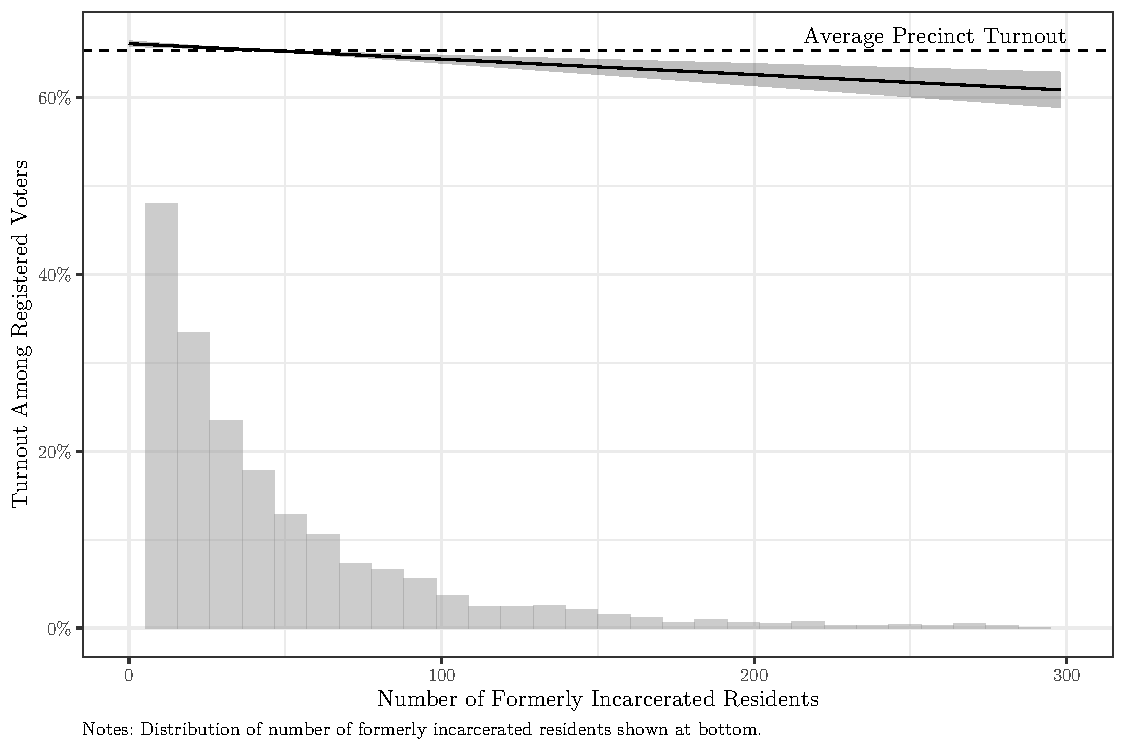
\includegraphics{amendment_4_turnout_files/figure-latex/marg1-1} 

}

\caption{\label{fig:marg1}Marginal Effect of Formerly Incarcerated Residents on Precinct Turnout Among Registered Voters}\label{fig:marg1}
\end{figure}

In Table \ref{tab:other-precincts} I present the results of OLS models that test whether the number of formerly incarcerated community members influenced a neighborhood's support for Amendment 4 or Amendment 4 roll-off. Roll-off is calculated as \(1 - \frac{Ballots\:Cast\:for\:Amendment\:4}{Ballots\:Cast\:in\:Contest\:with\:the\:Most\:Votes}\). It ranges from zero (if everyone who cast a ballot made a decision on the Amendment 4 question) to one (if no participants voted for or against Amendment 4). A lower number represents lower roll-off, indicating that the issue was more salient for participants.

\begin{singlespace}

\input{"../temp/precinct_other.tex"}
\end{singlespace}

Table \ref{tab:other-precincts} demonstrates that precincts with more formerly incarcerated residents supported Amendment 4 at slightly higher rates. Similarly, roll-off was lower in neighborhoods with more formerly incarcerated residents. Figures \ref{fig:marg-alt} and \ref{fig:marg-alt2} plot the marginal effect of each additional formerly incarcerated resident on a precinct's support for Amendment 4 (model 1), and the precinct's roll-off on Amendment 4 (model 3). These figures make clear that the number of formerly incarcerated residents has a relatively small impact on precinct support for its passage, and a relatively large impact on precinct level roll-off.

\begin{figure}[H]

{\centering 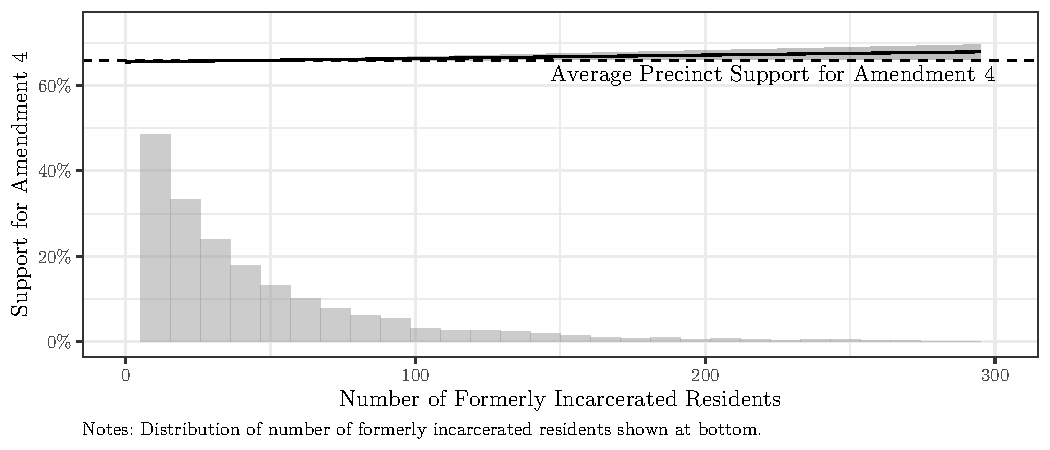
\includegraphics{amendment_4_turnout_files/figure-latex/marg-alt-1} 

}

\caption{\label{fig:marg-alt}Marginal Effect of Formerly Incarcerated Residents on Support for Amendment 4}\label{fig:marg-alt}
\end{figure}
\begin{figure}[H]

{\centering 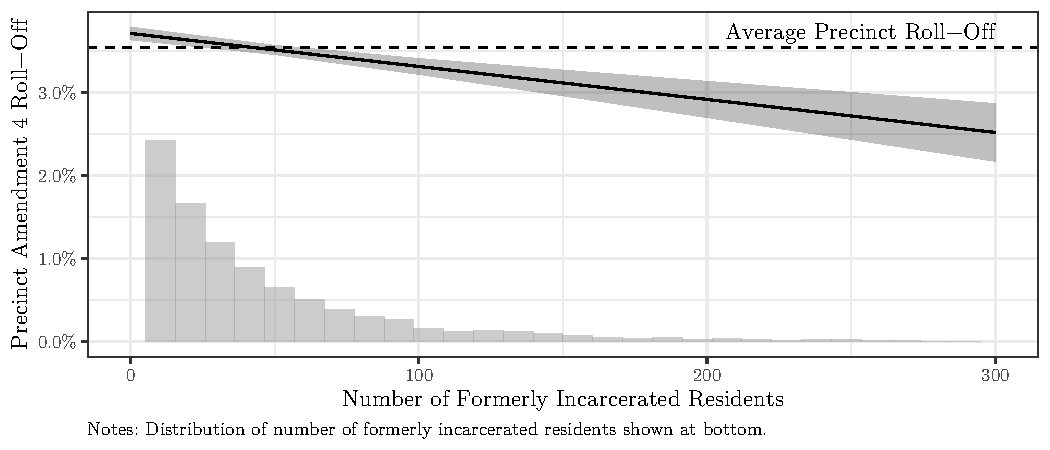
\includegraphics{amendment_4_turnout_files/figure-latex/marg-alt2-1} 

}

\caption{\label{fig:marg-alt2}Marginal Effect of Formerly Incarcerated Residents on Amendment 4 Roll-Off}\label{fig:marg-alt2}
\end{figure}

Why the relationship between formerly incarcerated residents and support is less strong (though positive and statistically significant) than salience is not clear, perhaps pointing to a variety of individual responses to crime and criminal justice policy in these neighborhoods. \protect\hyperlink{ref-Leverentz2011}{Leverentz} (\protect\hyperlink{ref-Leverentz2011}{2011}) argues that punitiveness is positively correlated with the salience of crime. The recently incarcerated residents might activate both punitiveness and support for the amendment, with support winning out slightly. The coefficients for \emph{Av. Years since Most Recent Incarceration} indicate that neighborhoods where the formerly incarcerated residents have been out of prison for longer saw both higher support for Amendment 4 and higher roll-off. Future work ought to interrogate how support for criminal justice reforms and the salience of those reforms change as community members' incarcerations recede into the past.

These neighborhood-level models demonstrate that neighborhoods with many formerly incarcerated residents did not turn out at higher rates than other, similar neighborhoods in 2018 even though Amendment 4 was on the ballot. However, while formerly incarcerated neighbors were not associated with getting people into the voting booth, they were associated with how voters cast their ballots once there.

\hypertarget{individual-level-results}{%
\subsection*{Individual-Level Results}\label{individual-level-results}}
\addcontentsline{toc}{subsection}{Individual-Level Results}

Neighborhood turnout rates could be obscuring underlying patterns. Inducements to vote at the household level might be too small to register at the neighborhood level, and it is possible that Amendment 4 shaped turnout differently for individuals who live with formerly incarcerated individuals than for their neighbors. A neighborhood may have disengaged from the political process thanks to exposure to the carceral state. Household members of the formerly incarcerated may have had a similar historical response, and yet be more susceptible to mobilization from Amendment 4; they are, after all, the voters whose identities are most likely shaped by indirect exposure to felony disenfranchisement.

This section directly examines the turnout of individuals who lived with formerly incarcerated individuals in 2018, relative to other, similar voters. As discussed above, I identify individuals who live with formerly incarcerated individuals by matching addresses listed in the Department of Corrections release data to the registered voter file. All registered voters who live at an address reported by a formerly incarcerated individual are considered ``treated.''

Each treated individual is then matched (\protect\hyperlink{ref-Sekhon2011}{Sekhon 2011}) with five untreated registered voters elsewhere in her congressional district.\footnote{Due to computing constraints, a random 5 percent random sample stratified by treatment status is used to calculate the genetic weights. The full sample is used for matching.} I use five matches in order to increase the sample size of the study; the large pool of potential controls means this can be done without sacrificing the quality of the matches. Voters' block group median income and share with some collegiate education come from the ACS 2018 5-year estimates, while all other characteristics come from the voter file. Matching is done with replacement and ties are not broken, which means that some treated voters may have more than five controls; the regression weights are calculated to allow for this possibility. Table \ref{tab:bal-table} presents the results of the matching exercise for each of the characteristics used.

\begin{singlespace}
\begin{table}[H]

\caption{\label{tab:balance-tab-chunk}\label{tab:bal-table} Balance Table}
\centering
\resizebox{\linewidth}{!}{
\begin{tabular}[t]{lllllrrrr}
\toprule
\multicolumn{1}{c}{ } & \multicolumn{2}{c}{Means: Unmatched Data} & \multicolumn{2}{c}{Means: Matched Data} & \multicolumn{4}{c}{Percent Improvement} \\
\cmidrule(l{3pt}r{3pt}){2-3} \cmidrule(l{3pt}r{3pt}){4-5} \cmidrule(l{3pt}r{3pt}){6-9}
 & Treated & Control & Treated & Control & Mean Diff & eQQ Med & eQQ Mean & eQQ Max\\
\midrule
\%White & 41.5\% & 63.2\% & 41.5\% & 41.5\% & 100.00 & 100.00 & 100.00 & 100.00\\
\% Black & 38.8\% & 12.7\% & 38.8\% & 38.8\% & 100.00 & 100.00 & 100.00 & 100.00\\
\% Latino & 12.8\% & 16.9\% & 12.8\% & 12.8\% & 100.00 & 100.00 & 100.00 & 100.00\\
\% Asian & 0.8\% & 2.0\% & 0.8\% & 0.8\% & 100.00 & 100.00 & 100.00 & 100.00\\
\% Female & 55.2\% & 52.4\% & 55.2\% & 55.2\% & 100.00 & 100.00 & 100.00 & 100.00\\
\% Male & 41.5\% & 45.0\% & 41.5\% & 41.5\% & 99.99 & 99.99 & 99.99 & 99.99\\
Registration Date & 2004-01-28 & 2004-09-24 & 2004-01-28 & 2004-02-11 & 94.03 & 38.85 & 27.88 & 19.19\\
Age & 48.95 & 52.45 & 48.95 & 48.77 & 94.71 & 94.34 & 92.44 & 90.89\\
\% Democrat & 53.7\% & 36.9\% & 53.7\% & 53.7\% & 99.99 & 99.99 & 99.99 & 99.99\\
\% Republican & 21.0\% & 35.4\% & 21.0\% & 21.0\% & 100.00 & 100.00 & 100.00 & 100.00\\
\% with Some College & 66.5\% & 75.3\% & 66.5\% & 66.5\% & 99.92 & 99.95 & 99.92 & 99.62\\
Median Income & \$47,389 & \$62,995 & \$47,389 & \$47,402 & 99.92 & 99.82 & 99.70 & 99.22\\
\bottomrule
\end{tabular}}
\end{table}
\end{singlespace}

As Table \ref{tab:bal-table} makes clear, the treated registered voters differ in meaningful ways from the rest of the electorate: three times as many are Black, a larger share are registered Democrats, and they live in neighborhoods with lower incomes. The matching process, however, results in a control group that is very similar to the treatment group with at least a 94 percent improvement in the mean difference for each measure.

Figure \ref{fig:dind} demonstrates that the parallel trends assumption is satisfied: although the treatment group has lower turnout rates in general, the gap between the treatment and control groups is largely constant between 2010 and 2016. Turnout in each year is measured as a function of voters registered in 2018, which partially explains why observed turnout is higher later in the period. Of course, some of the increase in turnout observed in later years in Figure \ref{fig:dind} can be attributed to higher ``real'' turnout as a share of eligible citizens.

\begin{figure}[H]

{\centering 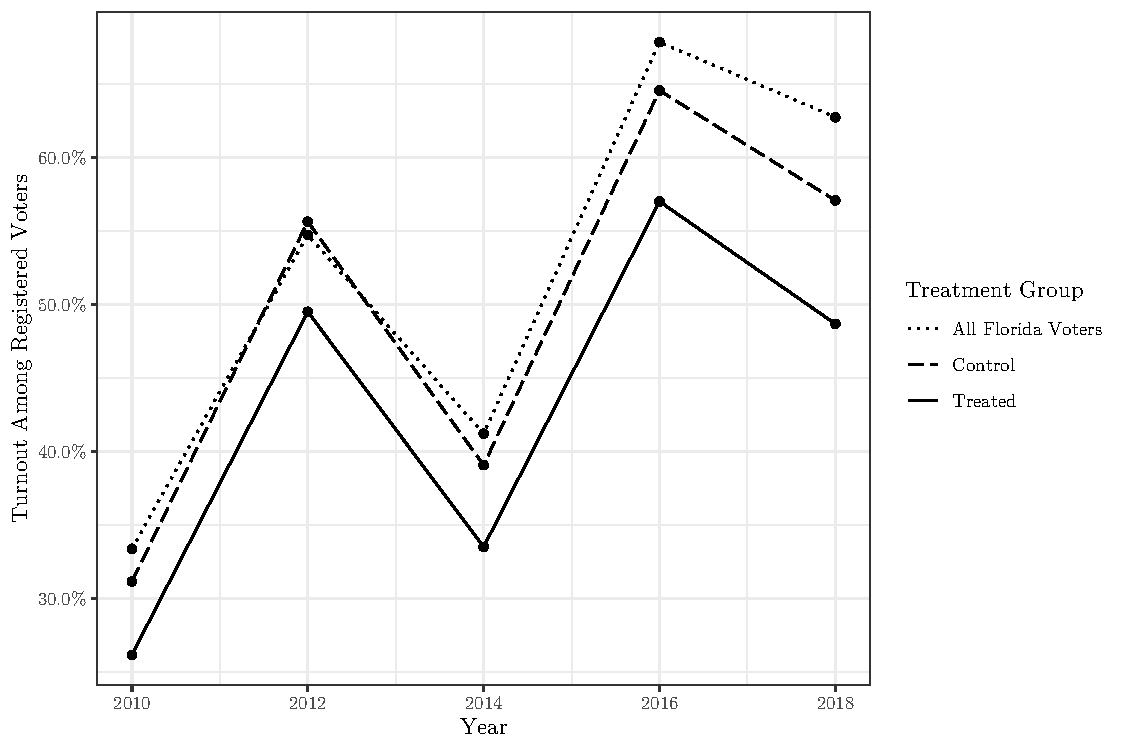
\includegraphics{amendment_4_turnout_files/figure-latex/dind-1} 

}

\caption{\label{fig:dind}General Election Turnout for Treated and Control Voters, 2010 -- 2018}\label{fig:dind}
\end{figure}

The trends presented in Figure \ref{fig:dind} offer preliminary visual corroboration of what I find at the neighborhood level --- namely, that 2018 turnout was not higher for voters in close contact with formerly incarcerated individuals. Table \ref{tab:tab-dind} formalizes these trends into an ordinary least squares regression.\footnote{Although the dependent variable here is binary --- it takes the value 0 if a voter does not participate, and 1 if she does --- the coefficients produced by logistic regressions in the difference-in-differences context are largely uninterpretable. I thus use a linear specification here. When the models are estimated using a logistic specification, the treatment effect is virtually identical.} A treatment dummy distinguishes treated from control voters. The treatment dummy is interacted with another dummy identifying the 2018 election. Robust standard errors are clustered at the level of the match (\protect\hyperlink{ref-Abadie2020}{Abadie and Spiess 2020}). Model 1 presents the model output without the other controls used for matching; model 2 includes these covariates.

In models 3 and 4 of Table \ref{tab:tab-dind} I consider the possibility that the negative spillover effects of incarceration dissipate over time. In these models, the dummies indicating treatment and the 2018 election are interacted with the number of years since the most recent release of a household member from prison (\emph{Years Since Latest Incarceration}, shortened to \emph{Years Since} in interactions). Matched control observations are assigned the value associated with their treated observation. Model 3 includes no other covariates, while model 4 includes the matched variables.

Formerly incarcerated individuals who were released from prison many years ago may no longer live at the same address they reported when leaving prison. Models 5 -- 8 therefore include only the treated individuals (and their matches) whose registration dates predate the latest prison release date of a household member, who we can be relatively sure lived with an incarcerated individual. The treatment effects in these models tell the same general story.

\begin{singlespace}
\input{"../temp/dind_reg_av.tex"}
\end{singlespace}

Each model in Table \ref{tab:tab-dind} identifies a negative treatment effect. The coefficients on \emph{2018 × Treated} in models 1 and 2 indicate that turnout among treated voters was about 2.2 percentage points below what it would have been if the gap between treated and control voters in 2018 had conformed to prior years. This mirrors the findings from the neighborhood-level analyses, where the number of formerly incarcerated residents is not associated with higher turnout.

There is some indication that spillover effects lessen with time. In each model, \emph{2018 × Treated × Years Since} and \emph{Treated × Years Since} is positive and statistically significant. In other words, individuals whose housemates had not been imprisoned for many years were more likely to vote than other treated voters, and this was especially true in 2018. Models 3 and 4 estimate that the treatment effect for an individual whose household member returned from prison within one year of the election was about -3.8 percentage points. For each year the most recent incarceration recedes into the past, the treatment effect decreases by about 0.2 points in years other than 2018, and by 0.4 points in 2018. That the spillover effects ``decay'' is a positive sign, and indicates that the negative socialization induced by a housemate's incarceration might not be permanent.

It is unsurprising that the effect is moderated by time. Individuals whose household members went to and were released from prison between the 2016 and 2018 elections, for instance, received two treatments: they both were ``negatively'' treated by the incarceration of their housemate and potentially ``positively'' treated by Amendment 4. What \emph{is} surprising, however, is the continued negative treatment effect even for the households furthest removed from the incarceration of a household member. Table \ref{tab:oldies} presents the results of models 5 and 6 from Table \ref{tab:tab-dind}, but limits the pool to households where someone last returned home from prison prior to 2010. The ``negative'' treatment for these individuals should be reflected in the base years of the difference-in-differences models. In these models, \emph{2018 × Treated} remains significant and negative. The neighborhood-level analyses indicate that the amount of time that has elapsed since an individual's incarceration is also related to support for and the salience of Amendment 4; similar processes may be at play here, but the individual-level data does not allow us to explore them.

\begin{singlespace}
\input{"../temp/dind_reg_medium_av.tex"}
\end{singlespace}

These negative, statistically significant findings at the individual and neighborhood level should probably not be interpreted to mean that Amendment 4 had a demobilizing effect on individuals whose family and community members would be re-enfranchised by its passage. Rather, it likely highlights that these individuals are less susceptible to other broadly mobilizing phenomena. The 2018 election saw higher participation than any midterm in a century as many infrequent voters turned out. It appears that voters whose household members have been to prison were less mobilized by the factors that encouraged other demographically similar voters to participate in 2018. This analysis cannot determine whether their indirect exposure to the criminal justice system caused this imperviousness, or if they would have remained on the sidelines in 2018 even if their household members had not been imprisoned. Nevertheless, that their turnout in 2018 did not increase relative to other voters --- even with Amendment 4 on the ballot --- underscores just how difficult their political (re)integration is.

\hypertarget{discussion-and-conclusion}{%
\subsection*{Discussion and Conclusion}\label{discussion-and-conclusion}}
\addcontentsline{toc}{subsection}{Discussion and Conclusion}

Turnout in 2018 hit historic levels for a midterm election as infrequent voters participated and made their voices heard. In addition to hotly contested Congressional, senate, and gubernatorial races, Floridians were presented with the opportunity to restore voting rights to well over a million permanently disenfranchised individuals who had been convicted of felony offenses. Amendment 4 and its organizers were hugely successful --- in a year where both statewide winners won by less than 0.5 percentage points, nearly two-thirds of Floridians supported expanding the franchise. Neighborhoods and voters most directly impacted by felony disenfranchisement gained meaningful political representation from the passage of the amendment, and one of the ``durable markers'' of their civil death was nullified. However, I fail to uncover evidence that Amendment 4 itself increased the turnout of neighborhoods and individuals in close proximity to the formerly incarcerated above-and-beyond the increases observed among other voters and in other communities.

It is not immediately apparent why Amendment 4 did not disproportionately heighten mobilization among these voters. The current study cannot tell whether it was an issue of lower political knowledge, or because the legal estrangement of the carceral state runs too deep for a single ballot initiative to overcome. However, if estrangement was the reason that the ballot initiative failed to mobilize these voters, this was likely only reinforced in the aftermath of the 2018 election. After the state constitution was amended to re-enfranchise their family members and neighbors, legislators rewrote the law to exclude them anew.

Just months after the 2018 election the Florida legislature passed a bill requiring disenfranchised individuals to pay off all court-ordered financial obligations before registering to vote, despite the fact that the state was incapable of determining how much any individual actually owed (\protect\hyperlink{ref-Stern2019}{Stern 2019}). A federal judge ruled the law unconstitutional in May of 2020, arguing that conditioning voting rights on the repayment of obligations that individuals cannot afford amounted to a poll tax and violation of the 24th Amendment.\footnote{Jones et al.~v. DeSantis et al., 4:19cv300-RH/MJF (U.S. District Court for the Northern District of Florida 2020).} That September, however, an en bank ruling by the U.S. Court of Appeals for the 11th Circuit overturned that decision,\footnote{Jones et al.~v. DeSantis et al., 4:19cv300-RH/MJF (United States Court of Appeals for the Eleventh Circuit).} upholding the constitutionality of the law. In his dissent from the Eleventh Circuit's ruling, Judge Adalberto Jordan noted that ``{[}h{]}ad Florida wanted to create a system to obstruct, impede, and impair the ability of felons to vote under Amendment 4, it could not have come up with a better one'' and that ``Florida cannot tell felons --- the great majority of whom are indigent --- how much they owe\ldots{} and has come up with conflicting (and uncodified) methods for determining how LFO {[}legal financial obligation{]} payments by felons should be credited.'' That Florida legislators would condition voting on criteria that cannot be verified, or cannot be afforded, has understandably been described as ``unfair {[}and{]} heartbreaking'' by one disenfranchised individual who said the amendment had promised to ``give me a voice in my own future'' (\protect\hyperlink{ref-Harris2020}{Harris 2020}). It remains to be seen how such legislation and litigation will inform how criminal justice-involved individuals understand their relationship with the state and structure their future democratic participation.

The results of this study point to the next chapter of the fight for political integration and representation for advocates in the Sunshine State. The relatively lower turnout in 2018 for the communities most impacted by the carceral state indicates that formal re-enfranchisement is not enough. If Floridian and American democracy wants to \emph{actually} incorporate voices from these communities --- and not simply legally \emph{allow} for their incorporation --- the advocacy movement cannot consider its work done once the formal barriers to the ballot box have been torn down. Re-enfranchisement is clearly necessary, but it is not sufficient. Researchers must continue exploring why the political re-incorporation of these communities is so difficult, and organizers on the ground must do the hard work of reknitting them to our body politic.

\newpage

\hypertarget{disclaimers}{%
\subsection*{Disclaimers}\label{disclaimers}}
\addcontentsline{toc}{subsection}{Disclaimers}

The author affirms this research did not directly involve human subjects.

The author declares no ethical issues or conflicts of interest in this research. This research was funded in part via the author's salary at the Brennan Center for Justice.

Research documentation and/or data that support the findings of this study are openly available in the APSR Dataverse at {[}DOI{]}. Limitations on data availability are discussed in the text and/or appendix.

\newpage

\hypertarget{references}{%
\subsection*{References}\label{references}}
\addcontentsline{toc}{subsection}{References}

\hypertarget{refs}{}
\begin{CSLReferences}{1}{0}
\leavevmode\hypertarget{ref-Abadie2020}{}%
Abadie, Alberto, and Jann Spiess. 2020. {``Robust {Post}-{Matching Inference}.''} \emph{Journal of the American Statistical Association} 0 (0): 1--13. \url{https://doi.org/10.1080/01621459.2020.1840383}.

\leavevmode\hypertarget{ref-Amos2020}{}%
Amos, Brian, and Michael P. McDonald. 2020. {``A {Method} to {Audit} the {Assignment} of {Registered Voters} to {Districts} and {Precincts}.''} \emph{Political Analysis} 28 (3): 356--71. \url{https://doi.org/10.1017/pan.2019.44}.

\leavevmode\hypertarget{ref-Amos2017}{}%
Amos, Brian, Michael P. McDonald, and Russell Watkins. 2017. {``When {Boundaries CollideConstructing} a {National Database} of {Demographic} and {Voting Statistics}.''} \emph{Public Opinion Quarterly} 81 (S1): 385--400. \url{https://doi.org/10.1093/poq/nfx001}.

\leavevmode\hypertarget{ref-Bell2017}{}%
Bell, Monica C. 2017. {``Police {Reform} and the {Dismantling} of {Legal Estrangement}.''} \emph{The Yale Law Journal} 126 (7): 2054--150. \url{http://www.jstor.org/stable/45222555}.

\leavevmode\hypertarget{ref-Bousquet2018a}{}%
Bousquet, Steve. 2018. {``Judge: {Florida}'s Early Voting-on-Campus Ban Shows {`Stark Pattern of Discrimination'}.''} \emph{Tampa Bay Times}, July 24, 2018. \url{https://www.tampabay.com/florida-politics/buzz/2018/07/24/judge-faults-state-and-approves-early-voting-on-college-university-campuses/}.

\leavevmode\hypertarget{ref-Bowers2009}{}%
Bowers, Melanie, and Robert R. Preuhs. 2009. {``Collateral {Consequences} of a {Collateral Penalty}: {The Negative Effect} of {Felon Disenfranchisement Laws} on the {Political Participation} of {Nonfelons}.''} \emph{Social Science Quarterly} 90 (3): 722--43. \url{https://doi.org/10.1111/j.1540-6237.2009.00640.x}.

\leavevmode\hypertarget{ref-Bowler1994}{}%
Bowler, Shaun, and Todd Donovan. 1994. {``Information and {Opinion Change} on {Ballot Propositions}.''} \emph{Political Behavior} 16 (4): 411--35. \url{http://www.jstor.org/stable/586468}.

\leavevmode\hypertarget{ref-Brayne2014}{}%
Brayne, Sarah. 2014. {``Surveillance and {System Avoidance}: {Criminal Justice Contact} and {Institutional Attachment}.''} \emph{American Sociological Review} 79 (3): 367--91. \url{https://doi.org/10.1177/0003122414530398}.

\leavevmode\hypertarget{ref-Burch2011}{}%
Burch, Traci R. 2011. {``Turnout and {Party Registration} Among {Criminal Offenders} in the 2008 {General Election}.''} \emph{Law \& Society Review} 45 (3): 699--730. \url{https://doi.org/10.1111/j.1540-5893.2011.00448.x}.

\leavevmode\hypertarget{ref-Burch2014}{}%
---------. 2014. {``Effects of {Imprisonment} and {Community Supervision} on {Neighborhood Political Participation} in {North Carolina}:''} \emph{The ANNALS of the American Academy of Political and Social Science} 651 (1): 184--201. \url{https://doi.org/10.1177/0002716213503093}.

\leavevmode\hypertarget{ref-Colgan2019}{}%
Colgan, Beth A. 2019. {``Wealth-{Based Penal Disenfranchisement}.''} \emph{Vanderbilt Law Review}, 55-189, 72 (1). https://doi.org/\url{https://scholarship.law.vanderbilt.edu/vlr/vol72/iss1/2}.

\leavevmode\hypertarget{ref-Comfort2016}{}%
Comfort, Megan. 2016. {``{`{A Twenty}-{Hour}-a-{Day Job}'}: {The Impact} of {Frequent Low}-{Level Criminal Justice Involvement} on {Family Life}.''} \emph{The ANNALS of the American Academy of Political and Social Science} 665 (1): 63--79. \url{https://doi.org/10.1177/0002716215625038}.

\leavevmode\hypertarget{ref-Ewald2002}{}%
Ewald, Alec C. 2002. {``'{Civil} Death': {The} Ideological Paradox of Criminal Disenfranchisement Law in the {United States}.''} \emph{Wisconsin Law Review} 2002 (5): 1045--1137.

\leavevmode\hypertarget{ref-Fairdosi2015}{}%
Fairdosi, Amir Shawn, and Jon C. Rogowski. 2015. {``Candidate {Race}, {Partisanship}, and {Political Participation}: {When Do Black Candidates Increase Black Turnout}?''} \emph{Political Research Quarterly} 68 (2): 337--49. \url{https://doi.org/10.1177/1065912915577819}.

\leavevmode\hypertarget{ref-Gelman2007}{}%
Gelman, Andrew, Jeffrey Fagan, and Alex Kiss. 2007. {``An {Analysis} of the {New York City Police Department}'s {`{Stop}-and-{Frisk}'} {Policy} in the {Context} of {Claims} of {Racial Bias}.''} \emph{Journal of the American Statistical Association} 102 (479): 813--23. \url{https://doi.org/10.1198/016214506000001040}.

\leavevmode\hypertarget{ref-Gerber2017}{}%
Gerber, Alan S., Gregory A. Huber, Marc Meredith, Daniel R. Biggers, and David J. Hendry. 2017. {``Does {Incarceration Reduce Voting}? {Evidence} about the {Political Consequences} of {Spending Time} in {Prison}.''} \emph{The Journal of Politics} 79 (4): 1130--46. \url{https://doi.org/10.1086/692670}.

\leavevmode\hypertarget{ref-Harris2020}{}%
Harris, Alex. 2020. {``Losing vote after Amendment 4 win is unfair, heartbreaking.''} \emph{Orlando Sentinel}, August 7, 2020. \url{https://www.orlandosentinel.com/opinion/guest-commentary/os-op-limiting-amendment-4-is-a-setback-20200807-hvcef76xongytccvyivu7o4s3y-story.html}.

\leavevmode\hypertarget{ref-Haskins2017}{}%
Haskins, Anna R., and Wade C. Jacobsen. 2017. {``Schools as {Surveilling Institutions}? {Paternal Incarceration}, {System Avoidance}, and {Parental Involvement} in {Schooling}.''} \emph{American Sociological Review} 82 (4): 657--84. \url{https://doi.org/10.1177/0003122417709294}.

\leavevmode\hypertarget{ref-Henig1994}{}%
Henig, Jeffrey R. 1994. {``To {Know Them Is} to ...? {Proximity} to {Shelters} and {Support} for the {Homeless}.''} \emph{Social Science Quarterly} 75 (4): 741--54. \url{http://www.jstor.org/stable/42863400}.

\leavevmode\hypertarget{ref-Justice2014}{}%
Justice, Benjamin, and Tracey L. Meares. 2014. {``How the {Criminal Justice System Educates Citizens}.''} \emph{The ANNALS of the American Academy of Political and Social Science} 651 (1): 159--77. \url{https://doi.org/10.1177/0002716213502929}.

\leavevmode\hypertarget{ref-Kelso2018}{}%
Kelso, Nathaniel, and Michael Migurski. 2018. {``Election-Geodata.''} {election-geodata}. 2018. \url{https://github.com/nvkelso/election-geodata}.

\leavevmode\hypertarget{ref-King2016}{}%
King, Bridgett A., and Laura Erickson. 2016. {``Disenfranchising the {Enfranchised}: {Exploring} the {Relationship Between Felony Disenfranchisement} and {African American Voter Turnout}.''} \emph{Journal of Black Studies} 47 (8): 799--821. \url{https://doi.org/10.1177/0021934716659195}.

\leavevmode\hypertarget{ref-Kirk2016}{}%
Kirk, David S. 2016. {``Prisoner {Reentry} and the {Reproduction} of {Legal Cynicism}.''} \emph{Social Problems} 63 (2): 222--43. \url{https://doi.org/10.1093/socpro/spw003}.

\leavevmode\hypertarget{ref-Kirk2011}{}%
Kirk, David S., and Mauri Matsuda. 2011. {``Legal {Cynicism}, {Collective Efficacy}, and the {Ecology} of {Arrest}.''} \emph{Criminology} 49 (2): 443--72. \url{https://doi.org/10.1111/j.1745-9125.2011.00226.x}.

\leavevmode\hypertarget{ref-Kirk2011a}{}%
Kirk, David S., and Andrew V. Papachristos. 2011. {``Cultural {Mechanisms} and the {Persistence} of {Neighborhood Violence}.''} \emph{American Journal of Sociology} 116 (4): 1190--1233. \url{https://doi.org/10.1086/655754}.

\leavevmode\hypertarget{ref-Lee2014}{}%
Lee, Hedwig, Lauren C. Porter, and Megan Comfort. 2014. {``Consequences of {Family Member Incarceration}: {Impacts} on {Civic Participation} and {Perceptions} of the {Legitimacy} and {Fairness} of {Government}.''} \emph{The ANNALS of the American Academy of Political and Social Science} 651 (1): 44--73. \url{https://doi.org/10.1177/0002716213502920}.

\leavevmode\hypertarget{ref-Lerman2014}{}%
Lerman, Amy E., and Vesla M. Weaver. 2014. \emph{Arresting Citizenship: The Democratic Consequences of {American} Crime Control}. Chicago Studies in {American} Politics. {Chicago}: {The University of Chicago Press}.

\leavevmode\hypertarget{ref-Leverentz2011}{}%
Leverentz, Andrea. 2011. {``Neighborhood Context of Attitudes Toward Crime and Reentry.''} \emph{Punishment \& Society} 13 (1): 64--92. \url{https://doi.org/10.1177/1462474510385629}.

\leavevmode\hypertarget{ref-McDonald2002}{}%
McDonald, Michael P. 2002. {``The {Turnout Rate} Among {Eligible Voters} in the {States}, 1980--2000.''} \emph{State Politics \& Policy Quarterly} 2 (2): 199--212. \url{https://doi.org/10.1177/153244000200200205}.

\leavevmode\hypertarget{ref-Meares2017}{}%
Meares, Tracey. 2017. {``Policing and {Procedural Justice}: {Shaping Citizens}' {Identities} to {Increase Democratic Participation}.''} \emph{Northwestern University Law Review} 111 (6): 1525--36.

\leavevmode\hypertarget{ref-Meredith2014}{}%
Meredith, Marc, and Michael Morse. 2014. {``Do {Voting Rights Notification Laws Increase Ex}-{Felon Turnout}?:''} \emph{The ANNALS of the American Academy of Political and Social Science} 651 (1): 220--49. \url{https://doi.org/10.1177/0002716213502931}.

\leavevmode\hypertarget{ref-Meredith2015}{}%
---------. 2015. {``The {Politics} of the {Restoration} of {Ex}-{Felon Voting Rights}: {The Case} of {Iowa}.''} \emph{Quarterly Journal of Political Science} 10 (1): 41--100. \url{https://doi.org/10.1561/100.00013026}.

\leavevmode\hypertarget{ref-Merolla2013}{}%
Merolla, Jennifer L., Abbylin H. Sellers, and Derek J. Fowler. 2013. {``Descriptive {Representation}, {Political Efficacy}, and {African Americans} in the 2008 {Presidential Election}.''} \emph{Political Psychology} 34 (6): 863--75. \url{https://doi.org/10.1111/j.1467-9221.2012.00934.x}.

\leavevmode\hypertarget{ref-Miles2004}{}%
Miles, Thomas J. 2004. {``Felon {Disenfranchisement} and {Voter Turnout}.''} \emph{The Journal of Legal Studies} 33 (1): 85--129. \url{https://doi.org/10.1086/381290}.

\leavevmode\hypertarget{ref-Miller2012}{}%
Miller, Bryan Lee, and Joseph F. Spillane. 2012a. {``Civil Death: {An} Examination of Ex-Felon Disenfranchisement and Reintegration.''} \emph{Punishment \& Society} 14 (4): 402--28. \url{https://doi.org/10.1177/1462474512452513}.

\leavevmode\hypertarget{ref-Miller2012a}{}%
---------. 2012b. {``Governing the Restoration of Civil Rights for Ex-Felons: An Evaluation of the {Executive Clemency Board} in {Florida}.''} \emph{Contemporary Justice Review} 15 (4): 413--34. \url{https://doi.org/10.1080/10282580.2012.734568}.

\leavevmode\hypertarget{ref-Miller2018}{}%
Miller, Peter, and Neilan S. Chaturvedi. 2018. {``Get Out the Early Vote: Co-Ethnic Mobilization and Convenience Voting.''} \emph{Journal of Elections, Public Opinion and Parties} 28 (4): 399--423. \url{https://doi.org/10.1080/17457289.2018.1437545}.

\leavevmode\hypertarget{ref-Morenoff2014}{}%
Morenoff, Jeffrey D., and David J. Harding. 2014. {``Incarceration, {Prisoner Reentry}, and {Communities}.''} \emph{Annual Review of Sociology} 40 (1): 411--29. \url{https://doi.org/10.1146/annurev-soc-071811-145511}.

\leavevmode\hypertarget{ref-Morris2020}{}%
Morris, Kevin. 2020. {``Neighborhoods and {Felony Disenfranchisement}: {The Case} of {New York City}.''} \emph{Urban Affairs Review}, 1078087420921522. \url{https://doi.org/10.1177/1078087420921522}.

\leavevmode\hypertarget{ref-Morris2021}{}%
---------. 2021. {``Welcome {Home}---{Now Vote}! {Voting Rights Restoration} and {Postsupervision Participation}.''} \emph{Social Science Quarterly} 102 (1): 140--53. \url{https://doi.org/10.1111/ssqu.12901}.

\leavevmode\hypertarget{ref-ORLANDOSENTINEL2018}{}%
\emph{Orlando Sentinel}. 2018. {``Florida's {Election} 2018: {Our} Endorsements for Governor, {U}.{S}. {Senate}, {U}.{S}. {House} and the Amendments,''} October 19, 2018. \url{https://www.orlandosentinel.com/opinion/editorials/os-op-orlando-sentinel-endorsements-20181018-htmlstory.html\#amend4\%5D}.

\leavevmode\hypertarget{ref-Ramadan2018}{}%
Ramadan, Lulu, Mike Stucka, and Wayne Washington. 2018. {``Florida Felon Voting Rights: {Who} Got Theirs Back Under {Scott}?''} \emph{The Palm Beach Post}, October 25, 2018. \url{https://www.palmbeachpost.com/news/20181025/florida-felon-voting-rights-who-got-theirs-back-under-scott}.

\leavevmode\hypertarget{ref-Remster2018}{}%
Remster, Brianna, and Rory Kramer. 2018. {``Race, {Space}, and {Surveillance}: {Understanding} the {Relationship} Between {Criminal Justice Contact} and {Institutional Involvement}.''} \emph{Socius} 4 (January). \url{https://doi.org/10.1177/2378023118761434}.

\leavevmode\hypertarget{ref-Robles2018}{}%
Robles, Frances. 2018. {``1.4 {Million Floridians With Felonies Win Long}-{Denied Right} to {Vote}.''} \emph{The New York Times}, November 7, 2018. \url{https://www.nytimes.com/2018/11/07/us/florida-felon-voting-rights.html}.

\leavevmode\hypertarget{ref-Sampson1998}{}%
Sampson, Robert J., and Dawn Jeglum Bartusch. 1998. {``Legal {Cynicism} and ({Subcultural}?) {Tolerance} of {Deviance}: {The Neighborhood Context} of {Racial Differences}.''} \emph{Law \& Society Review} 32 (4): 777--804. \url{https://doi.org/10.2307/827739}.

\leavevmode\hypertarget{ref-Schlakman2018}{}%
Schlakman, Mark. 2018. {``Some Facts and Figures You Might Not Know about Civil Rights Restoration in {Florida}.''} \emph{Tampa Bay Times}, April 19, 2018. \url{https://www.tampabay.com/opinion/columns/Column-Some-facts-and-figures-you-might-not-know-about-civil-rights-restoration-in-Florida_167477194/}.

\leavevmode\hypertarget{ref-Sekhon2011}{}%
Sekhon, Jasjeet S. 2011. {``Multivariate and {Propensity Score Matching Software} with {Automated Balance Optimization}: {The Matching} Package for {R}.''} \emph{Journal of Statistical Software} 42 (7): 1--52. \url{https://doi.org/10.18637/jss.v042.i07}.

\leavevmode\hypertarget{ref-Shaker2012}{}%
Shaker, Lee. 2012. {``Local {Political Knowledge} and {Assessments} of {Citizen Competence}.''} \emph{Public Opinion Quarterly} 76 (3): 525--37. \url{https://doi.org/10.1093/poq/nfs018}.

\leavevmode\hypertarget{ref-Smith2018}{}%
Smith, Jamil. 2018. {``Andrew {Gillum Is Ready}. {Is Florida}?''} \emph{Rolling Stone}, October 31, 2018. \url{https://www.rollingstone.com/politics/politics-features/andrew-gillum-florida-governor-race-749651/}.

\leavevmode\hypertarget{ref-Speri2018}{}%
Speri, Alice. 2018. {``Florida's {Amendment} 4 {Would Restore Voting Rights} to 1.4 {Million People}.''} \emph{The Intercept}, November 3, 2018. \url{https://theintercept.com/2018/11/03/florida-felon-voting-rights-amendment-4/}.

\leavevmode\hypertarget{ref-Stern2019}{}%
Stern, Mark Joseph. 2019. {``Florida {Republicans Are Sabotaging} a {Constitutional Amendment That Gave Felons} the {Right} to {Vote}.''} \emph{Slate Magazine}, March 20, 2019. \url{https://slate.com/news-and-politics/2019/03/florida-republicans-felon-voting-rights-amendment-4.html}.

\leavevmode\hypertarget{ref-SunSentinelEditorial2018}{}%
\emph{Sun Sentinel}. 2018. {``Five good --- seven bad --- amendments for Florida's Constitution,''} October 5, 2018. \url{https://www.sun-sentinel.com/opinion/endorsements/fl-op-end-good-bad-constitutional-amendments-20181005-story.html}.

\leavevmode\hypertarget{ref-tampabaytimes2018}{}%
\emph{Tampa Bay Times}. 2018. {``Times Recommends: {Yes} on {Amendment} 4,''} October 3, 2018. \url{https://www.tampabay.com/opinion/editorials/times-recommends-yes-on-amendment-4-20180928/}.

\leavevmode\hypertarget{ref-Taylor2018}{}%
Taylor, Adam. 2018. {``Florida's Move to Allow Ex-Felons to Vote Brings {U}.{S}. Closer to International Election Norms.''} \emph{Washington Post}, November 7, 2018. \url{https://www.washingtonpost.com/world/2018/11/07/floridas-move-allow-ex-felons-vote-brings-us-closer-international-election-norms/}.

\leavevmode\hypertarget{ref-Tragos2008}{}%
Tragos, George E., and Peter A. Sartes. 2008. {``Withhold of {Adjudication}: {What Everyone Needs} to {Know}.''} \emph{The Florida Bar Journal} 82 (2): 48.

\leavevmode\hypertarget{ref-Travis2003}{}%
Travis, Jeremy, and Michelle Waul, eds. 2003. \emph{Prisoners Once Removed: The Impact of Incarceration and Reentry on Children, Families, and Communities}. {Washington, D.C}: {Urban Institute Press}.

\leavevmode\hypertarget{ref-sentencing_2016}{}%
Uggen, Christopher, Ryan Larson, and Sarah Shannon. 2016. {``6 {Million Lost Voters}: {State}-{Level Estimates} of {Felony Disenfranchisement}, 2016.''} Research report. {The Sentencing Project}. \url{https://www.sentencingproject.org/publications/6-million-lost-voters-state-level-estimates-felony-disenfranchisement-2016/}.

\leavevmode\hypertarget{ref-USPS2015}{}%
USPS. 2015. {``Appendix {C}.''} {Postal Addressing Standards}. May 2015. \url{https://pe.usps.com/text/pub28/28apc_002.htm}.

\leavevmode\hypertarget{ref-Walker2014}{}%
Walker, Hannah L. 2014. {``Extending the {Effects} of the {Carceral State}: {Proximal Contact}, {Political Participation}, and {Race}.''} \emph{Political Research Quarterly} 67 (4): 809/822. \url{https://doi.org/10.1177/1065912914542522}.

\leavevmode\hypertarget{ref-Walker2020}{}%
---------. 2020. {``Targeted: {The Mobilizing Effect} of {Perceptions} of {Unfair Policing Practices}.''} \emph{The Journal of Politics} 82 (1): 119--34. \url{https://doi.org/10.1086/705684}.

\leavevmode\hypertarget{ref-Walker2017}{}%
Walker, Hannah L., and Marcela García-Castañon. 2017. {``For {Love} and {Justice}: {The Mobilizing} of {Race}, {Gender}, and {Criminal Justice Contact}.''} \emph{Politics \& Gender} 13 (4): 541--68. \url{https://doi.org/10.1017/S1743923X17000198}.

\leavevmode\hypertarget{ref-Washington2006}{}%
Washington, Ebonya. 2006. {``How {Black Candidates Affect Voter Turnout}.''} \emph{The Quarterly Journal of Economics} 121 (3): 973--98. \url{http://www.jstor.org/stable/25098814}.

\leavevmode\hypertarget{ref-Weaver2010}{}%
Weaver, Vesla M., and Amy E. Lerman. 2010. {``Political {Consequences} of the {Carceral State}.''} \emph{American Political Science Review} 104 (4): 817--33. \url{https://doi.org/10.1017/S0003055410000456}.

\leavevmode\hypertarget{ref-White2019a}{}%
White, Ariel. 2019a. {``Family {Matters}? {Voting Behavior} in {Households} with {Criminal Justice Contact}.''} \emph{American Political Science Review} 113 (2): 607--13. \url{https://doi.org/10.1017/S0003055418000862}.

\leavevmode\hypertarget{ref-White2019}{}%
---------. 2019b. {``Misdemeanor {Disenfranchisement}? {The Demobilizing Effects} of {Brief Jail Spells} on {Potential Voters}.''} \emph{American Political Science Review} 113 (2): 311--24. \url{https://doi.org/10.1017/S000305541800093X}.

\end{CSLReferences}

\end{document}
